\documentclass[aspectratio=169]{beamer}

\usepackage[utf8]{inputenc}
\usepackage[T1]{fontenc}
\usepackage[english]{babel}
\usepackage{graphicx}
\usepackage{amsmath,amssymb}
\usepackage{tikz}
\usetikzlibrary{positioning,arrows.meta}
\usepackage{tabularx}
\usepackage{booktabs}

% --- PWr color scheme ---
\xdefinecolor{pwrone}{rgb}{0.6015625,0.203125,0.17578125}
\xdefinecolor{pwrtwo}{rgb}{0.94140625,0.81640625,0.6328125}
\mode<presentation>
{
    \usetheme{Warsaw}
    \setbeamercolor{structure}{fg=pwrone}
    \setbeamercolor*{palette primary}{use=structure,fg=pwrtwo,bg=pwrone}
    \setbeamercolor*{palette quaternary}{use=structure,fg=pwrone,bg=pwrtwo}
}
\usetheme{Warsaw}

% --- Frame counter in footer ---
\newcommand*\oldmacro{}
\let\oldmacro\insertshortauthor
\renewcommand*\insertshortauthor{%
    \leftskip=.3cm%
    \insertframenumber\,/\,\inserttotalframenumber\hfill\oldmacro%
}

\newcolumntype{C}{>{\centering\arraybackslash}X}

\title[Motzkin Neighborhood for PFSP]
{Motzkin Neighborhood Evaluation\\
in Iterated Local Search and Simulated Annealing\\
for the Permutational Flow Shop Problem}
\author[R.~Wojew\'odzki, W.~Bo\.zejko]
{Remigiusz Wojew\'odzki \and Wojciech Bo\.zejko}
\institute{
{\tt remigiusz.wojewodzki@gmail.com} \quad {\tt wojciech.bozejko@pwr.edu.pl}\\[1mm]

\includegraphics[height=8mm]{logo_PWR.png}
}
\date{SOCO 2026\vspace{8mm}}

\begin{document}

% ===== SLIDE 1: TITLE =====
\frame{\thispagestyle{empty}\titlepage}

% ===== SLIDE 2: OUTLINE =====
\begin{frame}{Outline}
    \tableofcontents
\end{frame}

% ===== SLIDE 3 =====
\section{Introduction}
\begin{frame}{Introduction}
    \textbf{Permutation Flow Shop Problem (PFSP)} --- $n$ jobs, $m$ machines, same order, minimize $C_{\max}$. NP-hard for $m \geq 3$.

    \vspace{0.4cm}
    Four classical neighborhoods compared inside ILS and SA:

    \vspace{0.2cm}
    \begin{center}
    \begin{tikzpicture}[scale=0.95]
        \node[draw,fill=pwrtwo,rounded corners,minimum width=2.6cm,minimum height=1.1cm,align=center] (a) at (0,0)   {\textbf{Adjacent}\\\scriptsize single swap};
        \node[draw,fill=pwrtwo,rounded corners,minimum width=2.6cm,minimum height=1.1cm,align=center] (f) at (3.3,0) {\textbf{Fibonacci}\\\scriptsize disjoint swaps};
        \node[draw,fill=pwrtwo,rounded corners,minimum width=2.6cm,minimum height=1.1cm,align=center] (d) at (6.6,0) {\textbf{Dynasearch}\\\scriptsize segment swaps};
        \node[draw,fill=pwrone!30,rounded corners,minimum width=2.6cm,minimum height=1.1cm,align=center] (m) at (9.9,0) {\textbf{\emph{Motzkin}}\\\scriptsize non-crossing arcs};
        \draw[->,thick] (a) -- (f); \draw[->,thick] (f) -- (d); \draw[->,thick] (d) -- (m);
        \node[below=2pt of a,font=\scriptsize] {cheap};
        \node[below=2pt of f,font=\scriptsize] {compound};
        \node[below=2pt of d,font=\scriptsize] {expensive};
        \node[below=2pt of m,font=\scriptsize,pwrone] {\textbf{this work}};
    \end{tikzpicture}
    \end{center}
\end{frame}

% ===== SLIDE 4 =====
\section{Motzkin Neighborhood}
\begin{frame}{Motzkin Numbers and Neighborhood Structure}
    \begin{columns}
        \begin{column}{.5\textwidth}
            Motzkin numbers $M_n$ count \emph{non-crossing} arc configurations on $n$ ordered points (isolated points allowed).

            \vspace{0.3cm}
            Example on 7 points --- arcs $(0,4),(2,3),(5,6)$:
            \begin{center}
            \begin{tikzpicture}[scale=0.85]
                \foreach \x in {0,1,2,3,4,5,6}
                    \fill (\x,0) circle (3pt) node[below=4pt] {\small\x};
                \draw[thick, pwrone] (0,0) to[bend left=55] (4,0);
                \draw[thick, pwrone] (2,0) to[bend left=70] (3,0);
                \draw[thick, pwrone] (5,0) to[bend left=70] (6,0);
            \end{tikzpicture}
            \end{center}
        \end{column}
        \begin{column}{.5\textwidth}
            \centering
            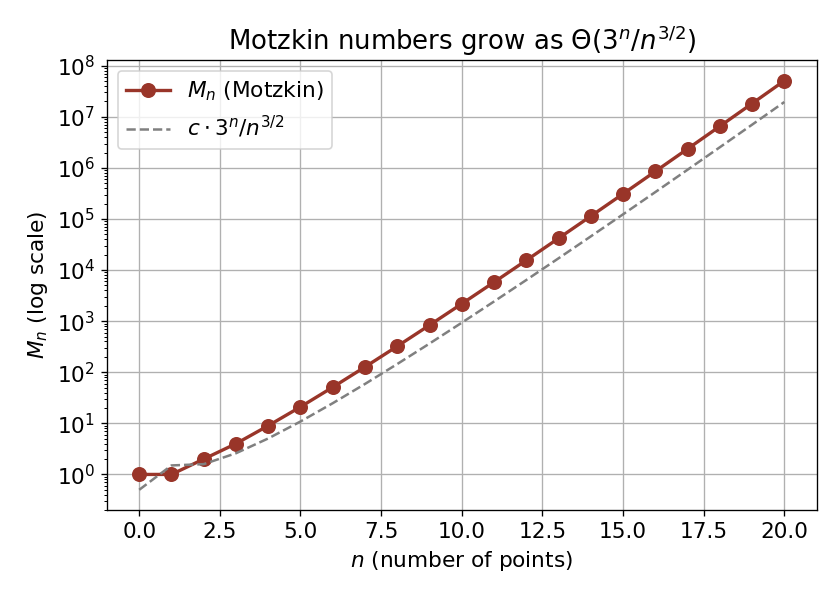
\includegraphics[width=\linewidth]{img/motzkin_growth.png}
        \end{column}
    \end{columns}
\end{frame}

% ===== SLIDE 5 =====
\begin{frame}{Admissibility Rules}
    A composite move $\mathcal{M} = \{(i_1,j_1),\dots,(i_k,j_k)\}$ is admissible iff:

    \vspace{0.3cm}
    \begin{center}
    \begin{tikzpicture}[scale=0.7]
        % Disjoint (OK)
        \begin{scope}[xshift=0cm]
            \foreach \x in {0,1,2,3,4,5} \fill (\x,0) circle (2pt);
            \draw[thick,pwrone] (0,0) to[bend left=60] (2,0);
            \draw[thick,pwrone] (3,0) to[bend left=60] (5,0);
            \node[below=10pt,font=\small,pwrone] at (2.5,-0.6) {\checkmark\ disjoint};
        \end{scope}
        % Crossing (NOT OK)
        \begin{scope}[xshift=8cm]
            \foreach \x in {0,1,2,3,4,5} \fill (\x,0) circle (2pt);
            \draw[thick,red!70] (0,0) to[bend left=60] (3,0);
            \draw[thick,red!70] (2,0) to[bend left=60] (5,0);
            \node[below=10pt,font=\small,red!70] at (2.5,-0.6) {$\times$\ crossing};
        \end{scope}
        % Nested (OK)
        \begin{scope}[xshift=16cm]
            \foreach \x in {0,1,2,3,4,5} \fill (\x,0) circle (2pt);
            \draw[thick,pwrone] (0,0) to[bend left=70] (5,0);
            \draw[thick,pwrone] (2,0) to[bend left=70] (3,0);
            \node[below=10pt,font=\small,pwrone] at (2.5,-0.6) {\checkmark\ nested};
        \end{scope}
    \end{tikzpicture}
    \end{center}

    \vspace{0.4cm}
    Plus \textbf{index disjointness}: $\{i_a,j_a\}\cap\{i_b,j_b\}=\varnothing$.

    \vspace{0.2cm}
    Each $(i,j)$ pair denotes an \emph{end swap} of segment $[\pi_i\dots\pi_j]$: only the endpoints exchange, the interior stays untouched.
\end{frame}

% ===== SLIDE 6 =====
\section{Algorithm}
\begin{frame}{Constructing the Best Composite Move}
    Single-iteration optimization via dynamic programming:
    \begin{enumerate}
        \item Compute Head and Tail completion-time matrices --- $O(mn)$.
        \item Evaluate all pairwise end-swap deltas $\Delta_{i,j}$ via Head$+$Tail --- $O(mn^2)$.
        \item DP picks optimal set of non-crossing, non-overlapping pairs --- $O(n^3)$.
        \item Apply selected swaps; recompute $C_{\max}$.
    \end{enumerate}

    \vspace{0.3cm}
    \textbf{Trade-off:} one Motzkin iteration explores up to $M_n$ configurations in $O(n^3)$ time --- fewer rich moves vs.\ many simple ones (Adjacent: $n{-}1$ swaps in $O(mn)$).
\end{frame}

% ===== SLIDE 7 =====
\section{Experiments}
\begin{frame}{Experimental Setup}
    \begin{itemize}
        \item Taillard instances, $n \in \{20, 50, 100, 200, 500\}$, $m \in \{5, 10, 20\}$ --- 12 instance classes.
        \item Time limits: $t_{\max} \in \{100, 500, 1000, 2000, 5000, 10000\}$~ms.
        \item ILS: tabu list $\tau_{\text{tabu}} = 10$.
        \item SA: $T_0 = 1000$, $T_{\min} = 1$, $\alpha = 0.95$, reheat $r = 1.5$, stagnation 500~ms.
        \item Compared neighborhoods: Adjacent, Fibonacci, Dynasearch, \emph{Motzkin}.
        \item Metric: mean RPD to lower bound.
    \end{itemize}
\end{frame}

% ===== SLIDE 8 =====
\begin{frame}{Results --- Gap vs.\ Time Limit}
    \begin{columns}
        \begin{column}{.5\textwidth}
            \centering
            
\includegraphics[width=\linewidth]{img/ils_gap.png}\\\small ILS
        \end{column}
        \begin{column}{.5\textwidth}
            \centering
            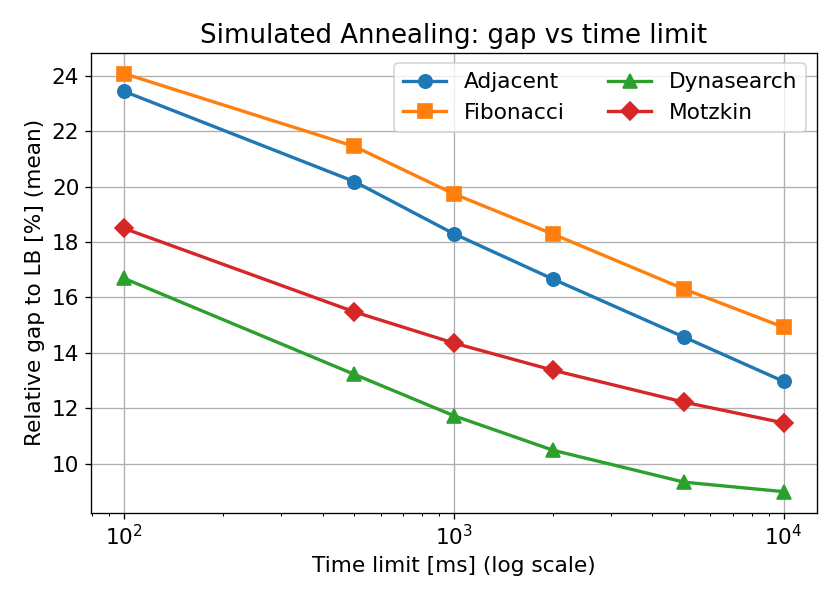
\includegraphics[width=\linewidth]{img/sa_gap.png}\\\small SA
        \end{column}
    \end{columns}

    \vspace{0.2cm}
    \centering\small \textbf{Dynasearch} lowest gap; \emph{Motzkin} beats Adjacent at larger $t_{\max}$; Fibonacci converges fastest but plateaus highest.
\end{frame}

% ===== SLIDE 9 =====
\begin{frame}{Statistical Significance (Wilcoxon signed-rank)}
    \centering
    \begin{tikzpicture}[scale=1]
        % Three vertical bars showing significance level
        \node[draw,fill=pwrone!80,minimum width=2.2cm,minimum height=3cm,align=center,text=white] (a) at (0,0)   {\textbf{Dynasearch}\\\small vs.\ all others\\[2pt]$p<0.01$\\\scriptsize all $t_{\max}$};
        \node[draw,fill=pwrone!50,minimum width=2.2cm,minimum height=2.2cm,align=center] (b) at (4,-0.4) {\textbf{Motzkin}\\\small vs.\ Fibonacci\\[2pt]$p<0.05$\\\scriptsize $t_{\max}\geq 5$\,s};
        \node[draw,fill=pwrtwo,minimum width=2.2cm,minimum height=1.6cm,align=center] (c) at (8,-0.7) {\textbf{Motzkin}\\\small vs.\ Adjacent\\[2pt]n.s.};
    \end{tikzpicture}

    \vspace{0.3cm}
    \small Competing effects: Motzkin runs few rich moves; Adjacent runs many simple ones. Their per-iteration gains tend to offset over the 12 instance classes (limited sample size).
\end{frame}

% ===== SLIDE 10 =====
\section{Conclusion}
\begin{frame}{Conclusion and Future Work}
    \textbf{Summary:}
    \begin{itemize}
        \item Motzkin: structured multi-swap neighborhood based on non-crossing arcs.
        \item DP enables $O(n^3)$ exploration of an exponentially large move set.
        \item Beats Adjacent at larger time budgets in both ILS and SA.
        \item Falls behind Dynasearch, which has a richer candidate set at lower cost.
    \end{itemize}

    \vspace{0.2cm}
    \textbf{Future work:}
    \begin{itemize}
        \item Improve computational efficiency to allow more iterations per budget.
        \item Quantum-assisted Motzkin evaluation (D-Wave QUBO, QAOA).
        \item Hybrid neighborhood strategies --- cyclic / adaptive selection.
    \end{itemize}
\end{frame}

\end{document}
